% Options for packages loaded elsewhere
\PassOptionsToPackage{unicode}{hyperref}
\PassOptionsToPackage{hyphens}{url}
%
\documentclass[
]{book}
\usepackage{amsmath,amssymb}
\usepackage{lmodern}
\usepackage{iftex}
\ifPDFTeX
  \usepackage[T1]{fontenc}
  \usepackage[utf8]{inputenc}
  \usepackage{textcomp} % provide euro and other symbols
\else % if luatex or xetex
  \usepackage{unicode-math}
  \defaultfontfeatures{Scale=MatchLowercase}
  \defaultfontfeatures[\rmfamily]{Ligatures=TeX,Scale=1}
\fi
% Use upquote if available, for straight quotes in verbatim environments
\IfFileExists{upquote.sty}{\usepackage{upquote}}{}
\IfFileExists{microtype.sty}{% use microtype if available
  \usepackage[]{microtype}
  \UseMicrotypeSet[protrusion]{basicmath} % disable protrusion for tt fonts
}{}
\makeatletter
\@ifundefined{KOMAClassName}{% if non-KOMA class
  \IfFileExists{parskip.sty}{%
    \usepackage{parskip}
  }{% else
    \setlength{\parindent}{0pt}
    \setlength{\parskip}{6pt plus 2pt minus 1pt}}
}{% if KOMA class
  \KOMAoptions{parskip=half}}
\makeatother
\usepackage{xcolor}
\usepackage{color}
\usepackage{fancyvrb}
\newcommand{\VerbBar}{|}
\newcommand{\VERB}{\Verb[commandchars=\\\{\}]}
\DefineVerbatimEnvironment{Highlighting}{Verbatim}{commandchars=\\\{\}}
% Add ',fontsize=\small' for more characters per line
\usepackage{framed}
\definecolor{shadecolor}{RGB}{248,248,248}
\newenvironment{Shaded}{\begin{snugshade}}{\end{snugshade}}
\newcommand{\AlertTok}[1]{\textcolor[rgb]{0.94,0.16,0.16}{#1}}
\newcommand{\AnnotationTok}[1]{\textcolor[rgb]{0.56,0.35,0.01}{\textbf{\textit{#1}}}}
\newcommand{\AttributeTok}[1]{\textcolor[rgb]{0.77,0.63,0.00}{#1}}
\newcommand{\BaseNTok}[1]{\textcolor[rgb]{0.00,0.00,0.81}{#1}}
\newcommand{\BuiltInTok}[1]{#1}
\newcommand{\CharTok}[1]{\textcolor[rgb]{0.31,0.60,0.02}{#1}}
\newcommand{\CommentTok}[1]{\textcolor[rgb]{0.56,0.35,0.01}{\textit{#1}}}
\newcommand{\CommentVarTok}[1]{\textcolor[rgb]{0.56,0.35,0.01}{\textbf{\textit{#1}}}}
\newcommand{\ConstantTok}[1]{\textcolor[rgb]{0.00,0.00,0.00}{#1}}
\newcommand{\ControlFlowTok}[1]{\textcolor[rgb]{0.13,0.29,0.53}{\textbf{#1}}}
\newcommand{\DataTypeTok}[1]{\textcolor[rgb]{0.13,0.29,0.53}{#1}}
\newcommand{\DecValTok}[1]{\textcolor[rgb]{0.00,0.00,0.81}{#1}}
\newcommand{\DocumentationTok}[1]{\textcolor[rgb]{0.56,0.35,0.01}{\textbf{\textit{#1}}}}
\newcommand{\ErrorTok}[1]{\textcolor[rgb]{0.64,0.00,0.00}{\textbf{#1}}}
\newcommand{\ExtensionTok}[1]{#1}
\newcommand{\FloatTok}[1]{\textcolor[rgb]{0.00,0.00,0.81}{#1}}
\newcommand{\FunctionTok}[1]{\textcolor[rgb]{0.00,0.00,0.00}{#1}}
\newcommand{\ImportTok}[1]{#1}
\newcommand{\InformationTok}[1]{\textcolor[rgb]{0.56,0.35,0.01}{\textbf{\textit{#1}}}}
\newcommand{\KeywordTok}[1]{\textcolor[rgb]{0.13,0.29,0.53}{\textbf{#1}}}
\newcommand{\NormalTok}[1]{#1}
\newcommand{\OperatorTok}[1]{\textcolor[rgb]{0.81,0.36,0.00}{\textbf{#1}}}
\newcommand{\OtherTok}[1]{\textcolor[rgb]{0.56,0.35,0.01}{#1}}
\newcommand{\PreprocessorTok}[1]{\textcolor[rgb]{0.56,0.35,0.01}{\textit{#1}}}
\newcommand{\RegionMarkerTok}[1]{#1}
\newcommand{\SpecialCharTok}[1]{\textcolor[rgb]{0.00,0.00,0.00}{#1}}
\newcommand{\SpecialStringTok}[1]{\textcolor[rgb]{0.31,0.60,0.02}{#1}}
\newcommand{\StringTok}[1]{\textcolor[rgb]{0.31,0.60,0.02}{#1}}
\newcommand{\VariableTok}[1]{\textcolor[rgb]{0.00,0.00,0.00}{#1}}
\newcommand{\VerbatimStringTok}[1]{\textcolor[rgb]{0.31,0.60,0.02}{#1}}
\newcommand{\WarningTok}[1]{\textcolor[rgb]{0.56,0.35,0.01}{\textbf{\textit{#1}}}}
\usepackage{longtable,booktabs,array}
\usepackage{calc} % for calculating minipage widths
% Correct order of tables after \paragraph or \subparagraph
\usepackage{etoolbox}
\makeatletter
\patchcmd\longtable{\par}{\if@noskipsec\mbox{}\fi\par}{}{}
\makeatother
% Allow footnotes in longtable head/foot
\IfFileExists{footnotehyper.sty}{\usepackage{footnotehyper}}{\usepackage{footnote}}
\makesavenoteenv{longtable}
\usepackage{graphicx}
\makeatletter
\def\maxwidth{\ifdim\Gin@nat@width>\linewidth\linewidth\else\Gin@nat@width\fi}
\def\maxheight{\ifdim\Gin@nat@height>\textheight\textheight\else\Gin@nat@height\fi}
\makeatother
% Scale images if necessary, so that they will not overflow the page
% margins by default, and it is still possible to overwrite the defaults
% using explicit options in \includegraphics[width, height, ...]{}
\setkeys{Gin}{width=\maxwidth,height=\maxheight,keepaspectratio}
% Set default figure placement to htbp
\makeatletter
\def\fps@figure{htbp}
\makeatother
\setlength{\emergencystretch}{3em} % prevent overfull lines
\providecommand{\tightlist}{%
  \setlength{\itemsep}{0pt}\setlength{\parskip}{0pt}}
\setcounter{secnumdepth}{5}
\usepackage{booktabs}
\ifLuaTeX
  \usepackage{selnolig}  % disable illegal ligatures
\fi
\usepackage[]{natbib}
\bibliographystyle{plainnat}
\IfFileExists{bookmark.sty}{\usepackage{bookmark}}{\usepackage{hyperref}}
\IfFileExists{xurl.sty}{\usepackage{xurl}}{} % add URL line breaks if available
\urlstyle{same} % disable monospaced font for URLs
\hypersetup{
  pdftitle={NHISS Example},
  hidelinks,
  pdfcreator={LaTeX via pandoc}}

\title{NHISS Example}
\author{}
\date{\vspace{-2.5em}}

\usepackage{amsthm}
\newtheorem{theorem}{Theorem}[chapter]
\newtheorem{lemma}{Lemma}[chapter]
\newtheorem{corollary}{Corollary}[chapter]
\newtheorem{proposition}{Proposition}[chapter]
\newtheorem{conjecture}{Conjecture}[chapter]
\theoremstyle{definition}
\newtheorem{definition}{Definition}[chapter]
\theoremstyle{definition}
\newtheorem{example}{Example}[chapter]
\theoremstyle{definition}
\newtheorem{exercise}{Exercise}[chapter]
\theoremstyle{definition}
\newtheorem{hypothesis}{Hypothesis}[chapter]
\theoremstyle{remark}
\newtheorem*{remark}{Remark}
\newtheorem*{solution}{Solution}
\begin{document}
\maketitle

{
\setcounter{tocdepth}{1}
\tableofcontents
}
\hypertarget{baseline-characteristic-table}{%
\chapter{Baseline characteristic table}\label{baseline-characteristic-table}}

Baseline tables show the characteristics of research subjects included in a study. A table characterizing baseline characteristics is so important that it's typically the first table that appears in any observational epidemiology (or clinical trial) manuscript, so it's commonly referred to as a ``Table 1''. The ``Table 1'' contain information about the mean and standard deviation(or median and IQR) for continue/scale variable, and proportion for categorical variable.\\

Baseline characteristic table should be created before imputaion, matching, or weighting.

\begin{longtable}[]{@{}l@{}}
\toprule()
\endhead
Using data \textbf{final\_db} \\
Outcome variable : \textbf{HTN} \\
Follow-up period : \textbf{DATEDIFF} \\
Exposure variable : \textbf{DM} \\
Covariates : \textbf{Age, Sex, SES, Region, BMI, CCI, Comorbidities(Dyslipidemia, Ischemic heart disease)} \\
\bottomrule()
\end{longtable}

\begin{Shaded}
\begin{Highlighting}[]
\DocumentationTok{\#\# load library}
\FunctionTok{library}\NormalTok{(moonBook)}
\FunctionTok{library}\NormalTok{(dplyr)}
\end{Highlighting}
\end{Shaded}

\begin{Shaded}
\begin{Highlighting}[]
\DocumentationTok{\#\# load data}
\NormalTok{final\_db }\OtherTok{\textless{}{-}} \FunctionTok{read.csv}\NormalTok{(}\StringTok{\textquotesingle{}Data/final\_db.csv\textquotesingle{}}\NormalTok{, }\AttributeTok{header=}\NormalTok{T)}
\end{Highlighting}
\end{Shaded}

\begin{Shaded}
\begin{Highlighting}[]
\DocumentationTok{\#\# formula}
\NormalTok{formula.bc }\OtherTok{\textless{}{-}} \FunctionTok{formula}\NormalTok{(DM }\SpecialCharTok{\textasciitilde{}}\NormalTok{ HTN }\SpecialCharTok{+}\NormalTok{ DATEDIFF }\SpecialCharTok{+}\NormalTok{ AGE }\SpecialCharTok{+}\NormalTok{ SEX }\SpecialCharTok{+}\NormalTok{ SES }\SpecialCharTok{+}\NormalTok{ REGION }\SpecialCharTok{+}\NormalTok{ BMI }\SpecialCharTok{+}\NormalTok{ CCI }\SpecialCharTok{+}\NormalTok{ DYS }\SpecialCharTok{+}\NormalTok{ IHD)}
\end{Highlighting}
\end{Shaded}

\begin{center}\rule{0.5\linewidth}{0.5pt}\end{center}

\begin{itemize}
\tightlist
\item
  Use \textbf{mytable()} function in \textbf{moonBook} package to create baseline characteristic tables.

  \begin{itemize}
  \tightlist
  \item
    method=1 : forces analysis as normal-distributed\\
  \item
    method=3 : performs a Shapiro-Wilk test to decide between normal or non-normal
  \end{itemize}
\end{itemize}

\hypertarget{baseline-characteristic-table-1}{%
\section{Baseline characteristic table}\label{baseline-characteristic-table-1}}

\begin{Shaded}
\begin{Highlighting}[]
\FunctionTok{mytable}\NormalTok{(formula.bc, }\AttributeTok{data=}\NormalTok{final\_db, }\AttributeTok{method=}\DecValTok{3}\NormalTok{) }
\end{Highlighting}
\end{Shaded}

\begin{verbatim}
## 
##               Descriptive Statistics by 'DM'             
## —————————————————————————————————————————————————————————— 
##                     0                    1             p  
##                 (N=2356)              (N=118)       
## —————————————————————————————————————————————————————————— 
##  HTN                                                 0.000
##    - 0        2215 (94.0%)           69 (58.5%)           
##    - 1         141 ( 6.0%)           49 (41.5%)           
##  DATEDIFF 1685.0 [835.5;2460.5] 963.5 [324.0;1690.0] 0.000
##  AGE        36.0 [22.0;48.0]      58.0 [50.0;68.0]   0.000
##  SEX                                                 0.903
##    - 1        1182 (50.2%)           58 (49.2%)           
##    - 2        1174 (49.8%)           60 (50.8%)           
##  SES                                                 0.393
##    - 1         668 (29.6%)           29 (25.2%)           
##    - 2         709 (31.4%)           34 (29.6%)           
##    - 3         883 (39.1%)           52 (45.2%)           
##  REGION                                              0.996
##    - 1        1160 (49.5%)           58 (49.2%)           
##    - 2         489 (20.9%)           25 (21.2%)           
##    - 3         694 (29.6%)           35 (29.7%)           
##  BMI        23.1 [21.0;25.2]      24.3 [22.6;26.1]   0.013
##  CCI                                                 0.001
##    - 0        1810 (76.8%)           80 (67.8%)           
##    - 1         433 (18.4%)           23 (19.5%)           
##    - 2         113 ( 4.8%)           15 (12.7%)           
##  DYS                                                 0.000
##    - 0        2285 (97.0%)          100 (84.7%)           
##    - 1         71 ( 3.0%)            18 (15.3%)           
##  IHD                                                 0.476
##    - 0        2340 (99.3%)          116 (98.3%)           
##    - 1         16 ( 0.7%)            2 ( 1.7%)            
## ——————————————————————————————————————————————————————————
\end{verbatim}

\hypertarget{baseline-characteristic-table_total}{%
\section{Baseline characteristic table\_total}\label{baseline-characteristic-table_total}}

\begin{Shaded}
\begin{Highlighting}[]
\NormalTok{tot1 }\OtherTok{\textless{}{-}}\NormalTok{ final\_db }\SpecialCharTok{\%\textgreater{}\%} \FunctionTok{mutate}\NormalTok{(}\AttributeTok{tmp=}\DecValTok{1}\NormalTok{)}
\NormalTok{tot2 }\OtherTok{\textless{}{-}}\NormalTok{ final\_db }\SpecialCharTok{\%\textgreater{}\%} \FunctionTok{mutate}\NormalTok{(}\AttributeTok{tmp=}\DecValTok{2}\NormalTok{)}
\NormalTok{tot3 }\OtherTok{\textless{}{-}} \FunctionTok{rbind}\NormalTok{(tot1,tot2)}

\FunctionTok{mytable}\NormalTok{(tmp }\SpecialCharTok{\textasciitilde{}}\NormalTok{ HTN }\SpecialCharTok{+}\NormalTok{ DATEDIFF }\SpecialCharTok{+}\NormalTok{ AGE }\SpecialCharTok{+}\NormalTok{ SEX }\SpecialCharTok{+}\NormalTok{ SES }\SpecialCharTok{+}\NormalTok{ REGION }\SpecialCharTok{+}\NormalTok{ BMI }\SpecialCharTok{+}\NormalTok{ CCI }\SpecialCharTok{+}\NormalTok{ DYS }\SpecialCharTok{+}\NormalTok{ IHD, }\AttributeTok{data=}\NormalTok{tot3, }\AttributeTok{method=}\DecValTok{3}\NormalTok{)}
\end{Highlighting}
\end{Shaded}

\begin{verbatim}
## 
##               Descriptive Statistics by 'tmp'             
## ——————————————————————————————————————————————————————————— 
##                     1                     2             p  
##                 (N=2474)              (N=2474)       
## ——————————————————————————————————————————————————————————— 
##  HTN                                                  1.000
##    - 0        2284 (92.3%)          2284 (92.3%)           
##    - 1         190 ( 7.7%)           190 ( 7.7%)           
##  DATEDIFF 1656.0 [811.0;2458.0] 1656.0 [811.0;2458.0] 1.000
##  AGE        36.0 [22.0;50.0]      36.0 [22.0;50.0]    1.000
##  SEX                                                  1.000
##    - 1        1240 (50.1%)          1240 (50.1%)           
##    - 2        1234 (49.9%)          1234 (49.9%)           
##  SES                                                  1.000
##    - 1         697 (29.3%)           697 (29.3%)           
##    - 2         743 (31.3%)           743 (31.3%)           
##    - 3         935 (39.4%)           935 (39.4%)           
##  REGION                                               1.000
##    - 1        1218 (49.5%)          1218 (49.5%)           
##    - 2         514 (20.9%)           514 (20.9%)           
##    - 3         729 (29.6%)           729 (29.6%)           
##  BMI        23.2 [21.0;25.3]      23.2 [21.0;25.3]    1.000
##  CCI                                                  1.000
##    - 0        1890 (76.4%)          1890 (76.4%)           
##    - 1         456 (18.4%)           456 (18.4%)           
##    - 2         128 ( 5.2%)           128 ( 5.2%)           
##  DYS                                                  1.000
##    - 0        2385 (96.4%)          2385 (96.4%)           
##    - 1         89 ( 3.6%)            89 ( 3.6%)            
##  IHD                                                  1.000
##    - 0        2456 (99.3%)          2456 (99.3%)           
##    - 1         18 ( 0.7%)            18 ( 0.7%)            
## ———————————————————————————————————————————————————————————
\end{verbatim}

\hypertarget{multiple-imputation}{%
\chapter{Multiple imputation}\label{multiple-imputation}}

Multiple imputation is a general approach to the problem of missing data. It aims to allow for the uncertainty about the missing data by creating several different plausible imputed data sets and appropriately combining results obtained from each of them.

Multiple imputation using chained equations (MICE) were performed to generate 10 imputed datasets. For the imputation model, predictive mean matching was used for continuous data and logistic regression was used for binary data.

\begin{longtable}[]{@{}l@{}}
\toprule()
\endhead
Using data \textbf{final\_db} \\
Outcome variable : \textbf{HTN} \\
Follow-up period : \textbf{DATEDIFF} \\
Exposure variable : \textbf{DM} \\
Covariates : \textbf{Age, Sex, SES, Region, BMI, CCI, Comorbidities(Dyslipidemia, Ischemic heart disease)} \\
\bottomrule()
\end{longtable}

\begin{Shaded}
\begin{Highlighting}[]
\DocumentationTok{\#\# load library}
\FunctionTok{library}\NormalTok{(mice)}
\FunctionTok{library}\NormalTok{(dplyr)}
\end{Highlighting}
\end{Shaded}

\begin{Shaded}
\begin{Highlighting}[]
\DocumentationTok{\#\# load data}
\NormalTok{final\_db }\OtherTok{\textless{}{-}} \FunctionTok{read.csv}\NormalTok{(}\StringTok{\textquotesingle{}Data/final\_db.csv\textquotesingle{}}\NormalTok{, }\AttributeTok{header=}\NormalTok{T)}
\end{Highlighting}
\end{Shaded}

\hypertarget{the-number-of-missing-values}{%
\section{The number of missing values}\label{the-number-of-missing-values}}

\begin{Shaded}
\begin{Highlighting}[]
\NormalTok{na\_count }\OtherTok{\textless{}{-}} \ControlFlowTok{function}\NormalTok{(data)\{}
\NormalTok{  num.na }\OtherTok{\textless{}{-}} \FunctionTok{colSums}\NormalTok{(}\FunctionTok{is.na}\NormalTok{(data))}
\NormalTok{  per.na }\OtherTok{\textless{}{-}} \FunctionTok{paste0}\NormalTok{(}\FunctionTok{round}\NormalTok{(}\FunctionTok{colSums}\NormalTok{(}\FunctionTok{is.na}\NormalTok{(data))}\SpecialCharTok{/}\FunctionTok{nrow}\NormalTok{(data) }\SpecialCharTok{*}\DecValTok{100}\NormalTok{,}\DecValTok{2}\NormalTok{),}\StringTok{"\%"}\NormalTok{)}
  
  \FunctionTok{return}\NormalTok{(}\FunctionTok{data.frame}\NormalTok{(}\AttributeTok{missing=}\FunctionTok{paste0}\NormalTok{(num.na,}\StringTok{"("}\NormalTok{,per.na,}\StringTok{")"}\NormalTok{),}\AttributeTok{row.names =} \FunctionTok{names}\NormalTok{(num.na)))}
\NormalTok{\}}

\FunctionTok{na\_count}\NormalTok{(final\_db)}
\end{Highlighting}
\end{Shaded}

\begin{verbatim}
##               missing
## RN_INDI         0(0%)
## DM              0(0%)
## INDEX_DT        0(0%)
## HTN             0(0%)
## FU_DT           0(0%)
## AGE             0(0%)
## SEX             0(0%)
## SES            99(4%)
## REGION      13(0.53%)
## BMI      1565(63.26%)
## CCI             0(0%)
## DYS             0(0%)
## IHD             0(0%)
## DATEDIFF        0(0%)
\end{verbatim}

\begin{itemize}
\tightlist
\item
  Use \textbf{mice()} function in \textbf{mice} package to deal with missing data.

  \begin{itemize}
  \tightlist
  \item
    m=10 refers to the number of imputed datasets. Five is the default value.
  \item
    Extract imputed data sets using \textbf{compleate()} function
  \end{itemize}
\end{itemize}

\hypertarget{imputation-for-missing-values}{%
\section{Imputation for missing values}\label{imputation-for-missing-values}}

\begin{Shaded}
\begin{Highlighting}[]
\DocumentationTok{\#\# Exclude subject ID, index date before imputation}
\NormalTok{dat\_mice }\OtherTok{\textless{}{-}}\NormalTok{ final\_db }\SpecialCharTok{\%\textgreater{}\%} \FunctionTok{select}\NormalTok{(}\SpecialCharTok{{-}}\NormalTok{RN\_INDI, }\SpecialCharTok{{-}}\NormalTok{INDEX\_DT, }\SpecialCharTok{{-}}\NormalTok{FU\_DT) }
\NormalTok{dat\_imp }\OtherTok{\textless{}{-}} \FunctionTok{mice}\NormalTok{(dat\_mice, }\AttributeTok{m=}\DecValTok{10}\NormalTok{, }\AttributeTok{seed=}\DecValTok{1}\NormalTok{)}
\end{Highlighting}
\end{Shaded}

\begin{verbatim}
## 
##  iter imp variable
##   1   1  SES  REGION  BMI
##   1   2  SES  REGION  BMI
##   1   3  SES  REGION  BMI
##   1   4  SES  REGION  BMI
##   1   5  SES  REGION  BMI
##   1   6  SES  REGION  BMI
##   1   7  SES  REGION  BMI
##   1   8  SES  REGION  BMI
##   1   9  SES  REGION  BMI
##   1   10  SES  REGION  BMI
##   2   1  SES  REGION  BMI
##   2   2  SES  REGION  BMI
##   2   3  SES  REGION  BMI
##   2   4  SES  REGION  BMI
##   2   5  SES  REGION  BMI
##   2   6  SES  REGION  BMI
##   2   7  SES  REGION  BMI
##   2   8  SES  REGION  BMI
##   2   9  SES  REGION  BMI
##   2   10  SES  REGION  BMI
##   3   1  SES  REGION  BMI
##   3   2  SES  REGION  BMI
##   3   3  SES  REGION  BMI
##   3   4  SES  REGION  BMI
##   3   5  SES  REGION  BMI
##   3   6  SES  REGION  BMI
##   3   7  SES  REGION  BMI
##   3   8  SES  REGION  BMI
##   3   9  SES  REGION  BMI
##   3   10  SES  REGION  BMI
##   4   1  SES  REGION  BMI
##   4   2  SES  REGION  BMI
##   4   3  SES  REGION  BMI
##   4   4  SES  REGION  BMI
##   4   5  SES  REGION  BMI
##   4   6  SES  REGION  BMI
##   4   7  SES  REGION  BMI
##   4   8  SES  REGION  BMI
##   4   9  SES  REGION  BMI
##   4   10  SES  REGION  BMI
##   5   1  SES  REGION  BMI
##   5   2  SES  REGION  BMI
##   5   3  SES  REGION  BMI
##   5   4  SES  REGION  BMI
##   5   5  SES  REGION  BMI
##   5   6  SES  REGION  BMI
##   5   7  SES  REGION  BMI
##   5   8  SES  REGION  BMI
##   5   9  SES  REGION  BMI
##   5   10  SES  REGION  BMI
\end{verbatim}

\begin{Shaded}
\begin{Highlighting}[]
\DocumentationTok{\#\# Create 10 imputed data}
\ControlFlowTok{for}\NormalTok{ (i }\ControlFlowTok{in} \DecValTok{1}\SpecialCharTok{:}\NormalTok{dat\_imp}\SpecialCharTok{$}\NormalTok{m)\{}
\NormalTok{  z }\OtherTok{\textless{}{-}} \FunctionTok{assign}\NormalTok{(}\FunctionTok{paste0}\NormalTok{(}\StringTok{\textquotesingle{}dat\_imp\textquotesingle{}}\NormalTok{,i),}\FunctionTok{complete}\NormalTok{(dat\_imp,i))}
  \FunctionTok{assign}\NormalTok{(}\FunctionTok{paste0}\NormalTok{(}\StringTok{\textquotesingle{}dat\_imp\textquotesingle{}}\NormalTok{,i),}\FunctionTok{cbind}\NormalTok{(z,final\_db }\SpecialCharTok{\%\textgreater{}\%} \FunctionTok{select}\NormalTok{(RN\_INDI))) }
\NormalTok{\}}

\DocumentationTok{\#\# list of 10 imputed data }
\NormalTok{dat\_imp\_list }\OtherTok{\textless{}{-}} \FunctionTok{list}\NormalTok{(dat\_imp1,dat\_imp2,dat\_imp3,dat\_imp4,dat\_imp5,dat\_imp6,dat\_imp7,dat\_imp8,dat\_imp9,dat\_imp10)}
\end{Highlighting}
\end{Shaded}

\begin{Shaded}
\begin{Highlighting}[]
\DocumentationTok{\#\# Save multiple imputation result}
\FunctionTok{save}\NormalTok{(dat\_imp,}\AttributeTok{file=}\StringTok{"Data/dat\_imp.RData"}\NormalTok{)}
\DocumentationTok{\#\# Save list for imputed data}
\FunctionTok{save}\NormalTok{(dat\_imp\_list,}\AttributeTok{file=}\StringTok{"Data/dat\_imp\_list.RData"}\NormalTok{)}
\end{Highlighting}
\end{Shaded}

\hypertarget{cross}{%
\chapter{Cross-references}\label{cross}}

Cross-references make it easier for your readers to find and link to elements in your book.

\hypertarget{chapters-and-sub-chapters}{%
\section{Chapters and sub-chapters}\label{chapters-and-sub-chapters}}

There are two steps to cross-reference any heading:

\begin{enumerate}
\def\labelenumi{\arabic{enumi}.}
\tightlist
\item
  Label the heading: \texttt{\#\ Hello\ world\ \{\#nice-label\}}.

  \begin{itemize}
  \tightlist
  \item
    Leave the label off if you like the automated heading generated based on your heading title: for example, \texttt{\#\ Hello\ world} = \texttt{\#\ Hello\ world\ \{\#hello-world\}}.
  \item
    To label an un-numbered heading, use: \texttt{\#\ Hello\ world\ \{-\#nice-label\}} or \texttt{\{\#\ Hello\ world\ .unnumbered\}}.
  \end{itemize}
\item
  Next, reference the labeled heading anywhere in the text using \texttt{\textbackslash{}@ref(nice-label)}; for example, please see Chapter \ref{cross}.

  \begin{itemize}
  \tightlist
  \item
    If you prefer text as the link instead of a numbered reference use: \protect\hyperlink{cross}{any text you want can go here}.
  \end{itemize}
\end{enumerate}

\hypertarget{captioned-figures-and-tables}{%
\section{Captioned figures and tables}\label{captioned-figures-and-tables}}

Figures and tables \emph{with captions} can also be cross-referenced from elsewhere in your book using \texttt{\textbackslash{}@ref(fig:chunk-label)} and \texttt{\textbackslash{}@ref(tab:chunk-label)}, respectively.

See Figure \ref{fig:nice-fig}.

\begin{Shaded}
\begin{Highlighting}[]
\FunctionTok{par}\NormalTok{(}\AttributeTok{mar =} \FunctionTok{c}\NormalTok{(}\DecValTok{4}\NormalTok{, }\DecValTok{4}\NormalTok{, .}\DecValTok{1}\NormalTok{, .}\DecValTok{1}\NormalTok{))}
\FunctionTok{plot}\NormalTok{(pressure, }\AttributeTok{type =} \StringTok{\textquotesingle{}b\textquotesingle{}}\NormalTok{, }\AttributeTok{pch =} \DecValTok{19}\NormalTok{)}
\end{Highlighting}
\end{Shaded}

\begin{figure}

{\centering 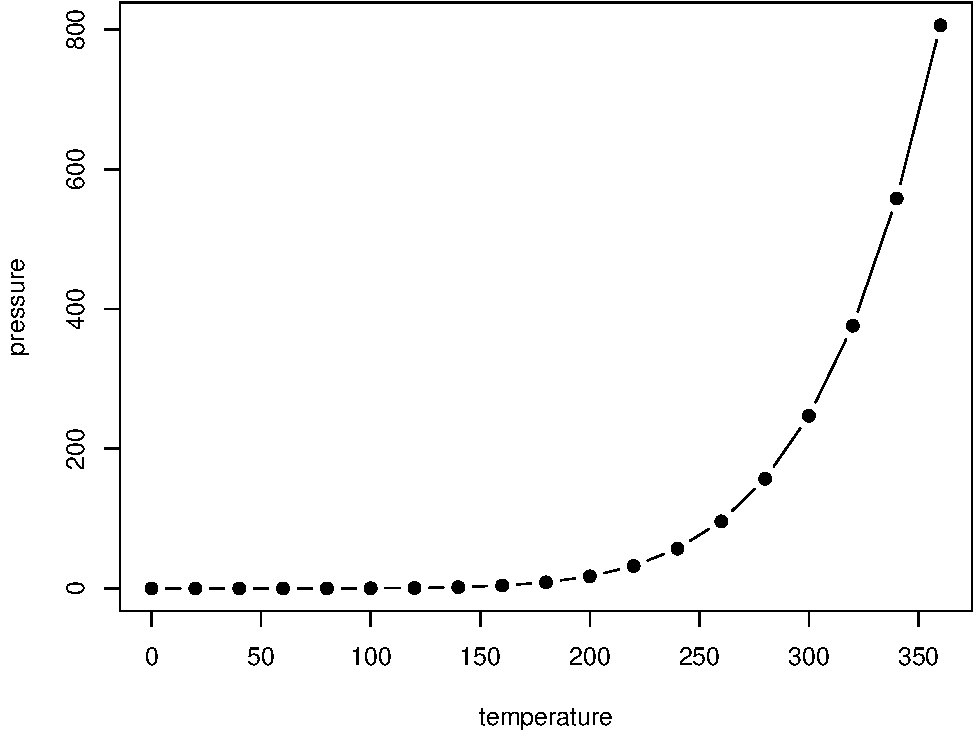
\includegraphics[width=0.8\linewidth]{bookdown_sample_files/figure-latex/nice-fig-1} 

}

\caption{Here is a nice figure!}\label{fig:nice-fig}
\end{figure}

Don't miss Table \ref{tab:nice-tab}.

\begin{Shaded}
\begin{Highlighting}[]
\NormalTok{knitr}\SpecialCharTok{::}\FunctionTok{kable}\NormalTok{(}
  \FunctionTok{head}\NormalTok{(pressure, }\DecValTok{10}\NormalTok{), }\AttributeTok{caption =} \StringTok{\textquotesingle{}Here is a nice table!\textquotesingle{}}\NormalTok{,}
  \AttributeTok{booktabs =} \ConstantTok{TRUE}
\NormalTok{)}
\end{Highlighting}
\end{Shaded}

\begin{table}

\caption{\label{tab:nice-tab}Here is a nice table!}
\centering
\begin{tabular}[t]{rr}
\toprule
temperature & pressure\\
\midrule
0 & 0.0002\\
20 & 0.0012\\
40 & 0.0060\\
60 & 0.0300\\
80 & 0.0900\\
\addlinespace
100 & 0.2700\\
120 & 0.7500\\
140 & 1.8500\\
160 & 4.2000\\
180 & 8.8000\\
\bottomrule
\end{tabular}
\end{table}

\hypertarget{parts}{%
\chapter{Parts}\label{parts}}

You can add parts to organize one or more book chapters together. Parts can be inserted at the top of an .Rmd file, before the first-level chapter heading in that same file.

Add a numbered part: \texttt{\#\ (PART)\ Act\ one\ \{-\}} (followed by \texttt{\#\ A\ chapter})

Add an unnumbered part: \texttt{\#\ (PART\textbackslash{}*)\ Act\ one\ \{-\}} (followed by \texttt{\#\ A\ chapter})

Add an appendix as a special kind of un-numbered part: \texttt{\#\ (APPENDIX)\ Other\ stuff\ \{-\}} (followed by \texttt{\#\ A\ chapter}). Chapters in an appendix are prepended with letters instead of numbers.

\hypertarget{footnotes-and-citations}{%
\chapter{Footnotes and citations}\label{footnotes-and-citations}}

\hypertarget{footnotes}{%
\section{Footnotes}\label{footnotes}}

Footnotes are put inside the square brackets after a caret \texttt{\^{}{[}{]}}. Like this one \footnote{This is a footnote.}.

\hypertarget{citations}{%
\section{Citations}\label{citations}}

Reference items in your bibliography file(s) using \texttt{@key}.

For example, we are using the \textbf{bookdown} package \citep{R-bookdown} (check out the last code chunk in index.Rmd to see how this citation key was added) in this sample book, which was built on top of R Markdown and \textbf{knitr} \citep{xie2015} (this citation was added manually in an external file book.bib).
Note that the \texttt{.bib} files need to be listed in the index.Rmd with the YAML \texttt{bibliography} key.

The RStudio Visual Markdown Editor can also make it easier to insert citations: \url{https://rstudio.github.io/visual-markdown-editing/\#/citations}

\hypertarget{blocks}{%
\chapter{Blocks}\label{blocks}}

\hypertarget{equations}{%
\section{Equations}\label{equations}}

Here is an equation.

\begin{equation} 
  f\left(k\right) = \binom{n}{k} p^k\left(1-p\right)^{n-k}
  \label{eq:binom}
\end{equation}

You may refer to using \texttt{\textbackslash{}@ref(eq:binom)}, like see Equation \eqref{eq:binom}.

\hypertarget{theorems-and-proofs}{%
\section{Theorems and proofs}\label{theorems-and-proofs}}

Labeled theorems can be referenced in text using \texttt{\textbackslash{}@ref(thm:tri)}, for example, check out this smart theorem \ref{thm:tri}.

\begin{theorem}
\protect\hypertarget{thm:tri}{}\label{thm:tri}For a right triangle, if \(c\) denotes the \emph{length} of the hypotenuse
and \(a\) and \(b\) denote the lengths of the \textbf{other} two sides, we have
\[a^2 + b^2 = c^2\]
\end{theorem}

Read more here \url{https://bookdown.org/yihui/bookdown/markdown-extensions-by-bookdown.html}.

\hypertarget{callout-blocks}{%
\section{Callout blocks}\label{callout-blocks}}

The R Markdown Cookbook provides more help on how to use custom blocks to design your own callouts: \url{https://bookdown.org/yihui/rmarkdown-cookbook/custom-blocks.html}

\hypertarget{sharing-your-book}{%
\chapter{Sharing your book}\label{sharing-your-book}}

\hypertarget{publishing}{%
\section{Publishing}\label{publishing}}

HTML books can be published online, see: \url{https://bookdown.org/yihui/bookdown/publishing.html}

\hypertarget{pages}{%
\section{404 pages}\label{pages}}

By default, users will be directed to a 404 page if they try to access a webpage that cannot be found. If you'd like to customize your 404 page instead of using the default, you may add either a \texttt{\_404.Rmd} or \texttt{\_404.md} file to your project root and use code and/or Markdown syntax.

\hypertarget{metadata-for-sharing}{%
\section{Metadata for sharing}\label{metadata-for-sharing}}

Bookdown HTML books will provide HTML metadata for social sharing on platforms like Twitter, Facebook, and LinkedIn, using information you provide in the \texttt{index.Rmd} YAML. To setup, set the \texttt{url} for your book and the path to your \texttt{cover-image} file. Your book's \texttt{title} and \texttt{description} are also used.

This \texttt{gitbook} uses the same social sharing data across all chapters in your book- all links shared will look the same.

Specify your book's source repository on GitHub using the \texttt{edit} key under the configuration options in the \texttt{\_output.yml} file, which allows users to suggest an edit by linking to a chapter's source file.

Read more about the features of this output format here:

\url{https://pkgs.rstudio.com/bookdown/reference/gitbook.html}

Or use:

\begin{Shaded}
\begin{Highlighting}[]
\NormalTok{?bookdown}\SpecialCharTok{::}\NormalTok{gitbook}
\end{Highlighting}
\end{Shaded}


  \bibliography{book.bib,packages.bib}

\end{document}
